\documentclass{article}
\usepackage[utf8]{inputenc}
\usepackage[euler]{textgreek}
\usepackage{amsmath}
\usepackage{amsfonts}
\usepackage{tabularx}
\usepackage{layout}
\usepackage{geometry}
\usepackage{calc}
\usepackage{siunitx}
\usepackage{graphicx}
\usepackage{listings}
\usepackage{xcolor}
\usepackage{longtable}
\usepackage{soul}
\usepackage{calligra}
\usepackage{mathtools}
\usepackage{float}
\usepackage{subfig}
\usepackage{physics}

\setlength{\hoffset}{0in}
\setlength{\voffset}{0in}
\setlength{\oddsidemargin}{0px}
\setlength{\headheight}{0em}
\setlength{\headsep}{0em}
\setlength{\marginparwidth}{0em}
\setlength{\marginparsep}{0em}
\setlength{\textheight}{\paperheight - 2in}
\setlength{\textwidth}{\paperwidth - 2in}
\setlength{\parskip}{1.5em}

\setlength{\parindent}{0px}
\setlength{\parskip}{2em}
\setlength{\tabcolsep}{0.2em}

\newcolumntype{C}{>{\centering\arraybackslash}X}

\newcommand{\hlc}[2][yellow]{{%
    \colorlet{foo}{#1}%
    \sethlcolor{foo}\hl{#2}}%
}

\newcommand*{\ZZ}{%
  \textsf{Z\kern-1ex Z}%
}

\newcommand{\question}[2]
{
    \begin{tabularx}{\linewidth}{lX}
        \textbf{#1)} & {#2}
    \end{tabularx} 
}

\newcommand{\silentquestion}[1]
{
    \begin{tabularx}{\linewidth}{lX}
        \phantom{\textbf{0)}} & {#1}
    \end{tabularx}
}

\newcommand{\expart}[1]
{
    \textbf{\underline{#1:}} \par 
}

% Pour les dx
\newcommand*\dif{\mathop{}\!\mathrm{d}}

% Pour faire dx/dt
\newcommand{\deriv}[1]{
    \frac{\dif #1}{\dif t}
}

\newcommand{\derivn}[2]{
    \frac{\dif^{#2} #1}{\dif t^{#2}}
}

% *10^x
\newcommand{\e}[1]{
    \times 10^{#1}
}

% Inclure du texte dans dans des environnements de maths avec des marges pas trop dégelasses
\newcommand{\txt}[1]{
    \;\text{#1}\;\;
}

% Unités
\newcommand{\un}[1]{
    \,\text{#1}
}

% Puissances pour unités, attention pour les lettres grecques il faut utiliser \text[letter] au lieu de \[letter]
\newcommand{\p}[1]{
    \!$^{#1}$\!\!\!
}

\begin{document}

\begin{tabularx}{\linewidth}{XCX}
    Chollet Arthur &\textbf{\underline{Compte rendu de la capacité numérique}}& 
\end{tabularx}

\expart{CN4 - Résolution d'une équation différentielle non-linéaire du 2nd ordre}
{
    \question{1}{
      \begin{itemize}
        \item \underline{Système:} M de masse m
        \item \underline{Référentielle} terrestre supposé galiléen
        \item \underline{Bilan des actions mécaniques:}
        
        $\vec{P}=m\vec{g}$ poids

        $\vec{T}$ tension du fil
        \item \underline{Schéma:}
        \begin{center}
          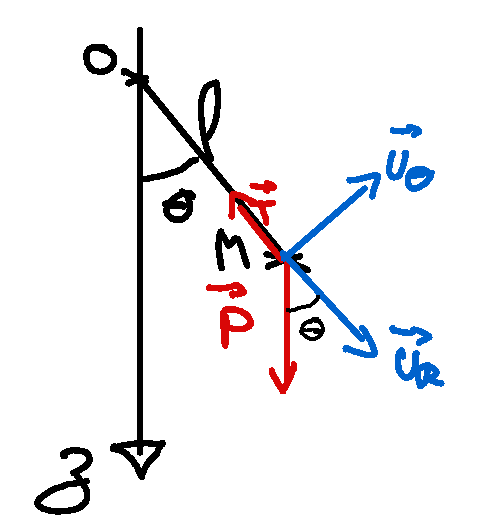
\includegraphics[height=12em]{images/CN4_schema.png}
        \end{center}

        \item \underline{Théorème de l'énergie cinétique:}
        \begin{align*}
          \dd E_c=\sum\delta W \txt{donc} \boxed{\dv{E_c}{t}=\sum\mathcal{P}}
        \end{align*} 
        Or en coordonnées polaire: \begin{align*}
          \vec{v}=\dot{r}\vec{u_r}+r\dot{\theta}\vec{u_{\theta}}
        \end{align*} 
        or $r=l=cst$ \begin{align*}
          \boxed{\vec{v}=l\dot{\theta}\vec{u_{\theta}} \txt{ ou} v=l\dot{\theta}}
        \end{align*}
        et \begin{align*}
          &\dv{E_c}{t}=\dv{(\frac{1}{2}mv^2)}{t}=\dv{(\frac{1}{2}ml^2\dot{\theta}^2)}{t}=\boxed{ml^2\dot{\theta}\ddot{\theta}}\\
          &\mathcal{P}(m\vec{g})=m\vec{g}\cdot\vec{v}=\boxed{-mgl\sin(\theta)\dot{\theta}}\\
          &\mathcal{P}(\vec{T})=\vec{T}\cdot\vec{v}=0
        \end{align*}
        ainsi \begin{align*}
          &ml^2\dot{\theta}\ddot{\theta}=-mgl\sin(\theta)\dot{\theta} \txt{ ou encore:}\\
          &\boxed{\ddot{\theta}+\frac{g}{l}\sin\theta=0} \txt{(en simpifiant les $\dot{\theta}$ car inutile au mouvement)}
        \end{align*}
      \end{itemize}
    }

    \question{2}{
      On pose: $u=\theta$ et $v=\dot{\theta}$

      Donc $\dot{u}=\dot{\theta}$ et $\dot{v}=\ddot{\theta}$

      Soit grâce à l'équation du mouvement:

      $\boxed{\begin{cases}
        \dot{u}=v \\
        \dot{v}=-\frac{g}{l}\sin u
      \end{cases}}$

      En testant nous obtenons des courbes cohérente avec la situation:
      \begin{figure}[H]
        \centering
        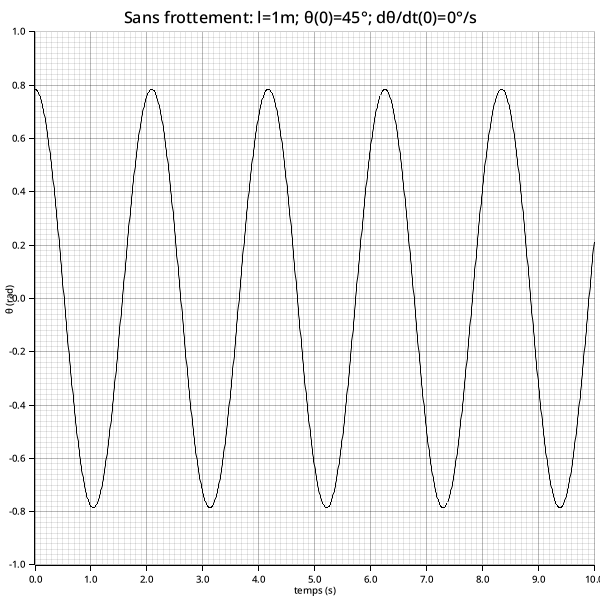
\includegraphics[width=20em]{images/pendule_45.png}
        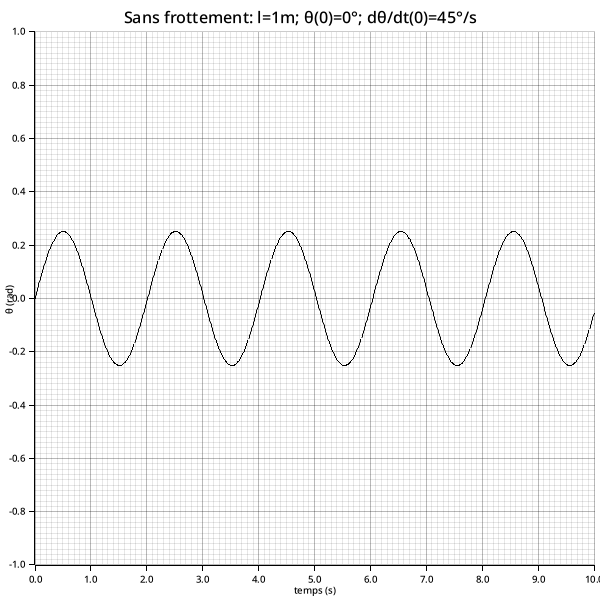
\includegraphics[width=20em]{images/pendule_0_vi.png}
        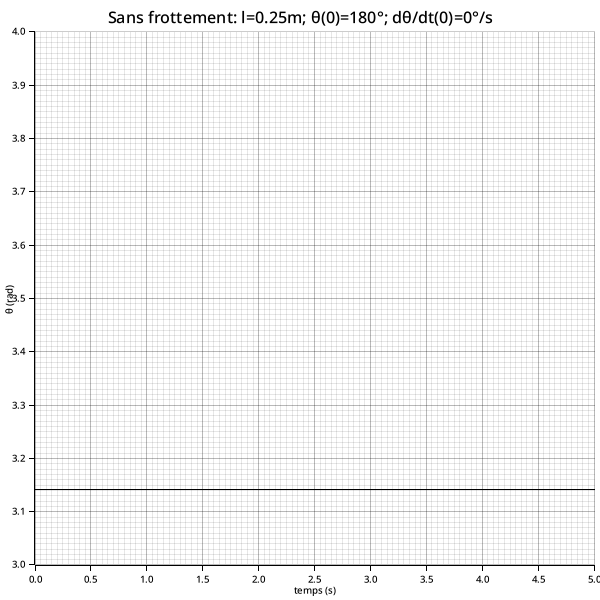
\includegraphics[width=20em]{images/pendule_180.png}
        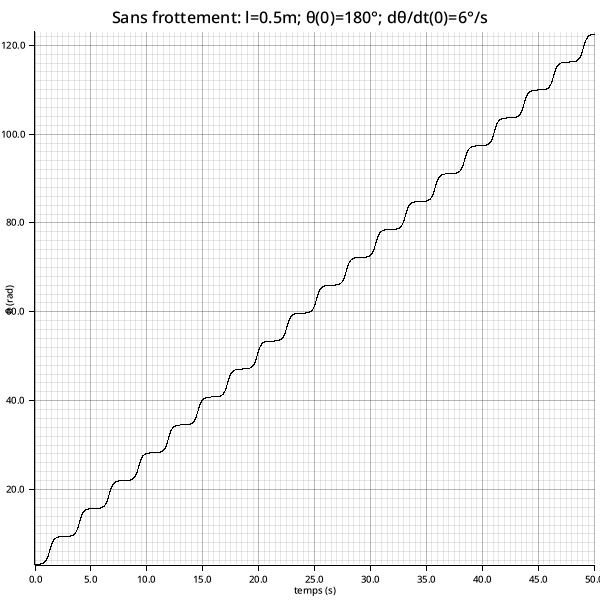
\includegraphics[width=20em]{images/pendule_180_vi.png}
        \caption{Quelque courbes simples}
    \end{figure}

    }

    \question{4}{
      D'après wikipédia on a la formule de borda à l'ordre 4:
      \begin{align*}
        \boxed{T=2\pi\sqrt{\frac{l}{g}}\left(1+\frac{\theta_0^2}{16}+\frac{11\theta_0^4}{3072}\right)}
      \end{align*}
      La formule à l'ordre 2 est valable jusqu'à $\approx\frac{\pi}{2}rad$, celle ci devrait donc être plus précise

      En utilisant l'algorithme de résolution de la question 2 et en déterminant les zéros de la solution (dichotomie), on peut en prenant 2 zéros séparé d'un autre retrouver la période du signal. En faisant ça pour un grand nombre de $\theta_0\in[0,\pi]$, nous obtenons la courbe noir suivante:
      \begin{figure}[H]
        \centering
        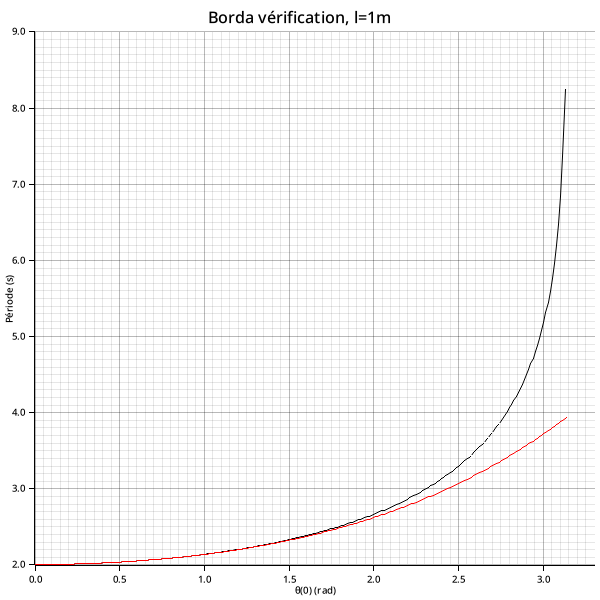
\includegraphics[width=35em]{images/borda.png}
        \caption{En noir l'approximation numérique. En orange la formule de borda à l'ordre 4}
      \end{figure}

      Nous voyons que pour les petits angles la formule de borda est entièrement égale à la vrai courbe, l'approximation est donc totalement juste, cependant à partir d'environ $2.0rad=115$\textdegree on remarque une erreur grandissante entre les 2 courbes, l'approximation devient fausses.
    }

    \question{5}{
      BONUS: avec frottement:

      grâce au PDF on trouve l'équation différentielle du mouvement:
      \begin{align*}
        \boxed{\ddot{\theta}+\frac{f}{m}\dot{\theta}+\frac{g}{l}\sin\theta=0} \txt{avec f coefficient de frottement fluide}
      \end{align*}
      De même, on pose $u=\theta$ et $v=\dot{\theta}$
      Donc $\dot{u}=\dot{\theta}$ et $\dot{v}=\ddot{\theta}$

      Soit grâce à l'équation du mouvement:

      $\boxed{\begin{cases}
        \dot{u}=v \\
        \dot{v}=-\frac{f}{m}v -\frac{g}{l}\sin u
      \end{cases}}$

      nous obtenons des courbes plus réaliste:
      \begin{figure}[H]
        \centering
        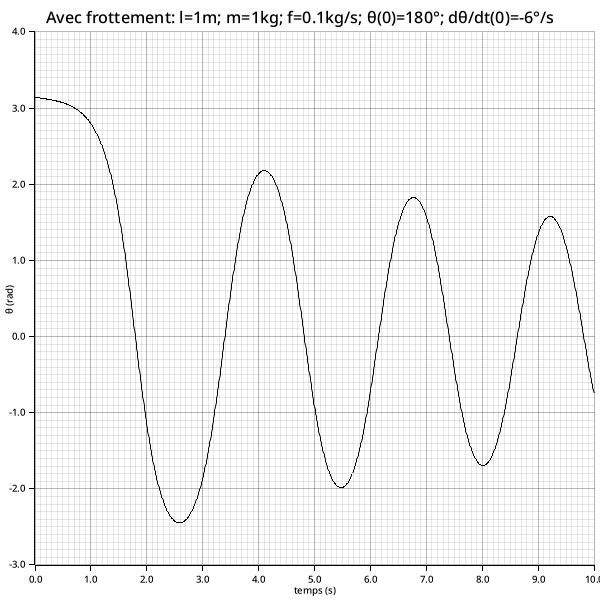
\includegraphics[width=20em]{images/pendule_friction_180_vi.png}
        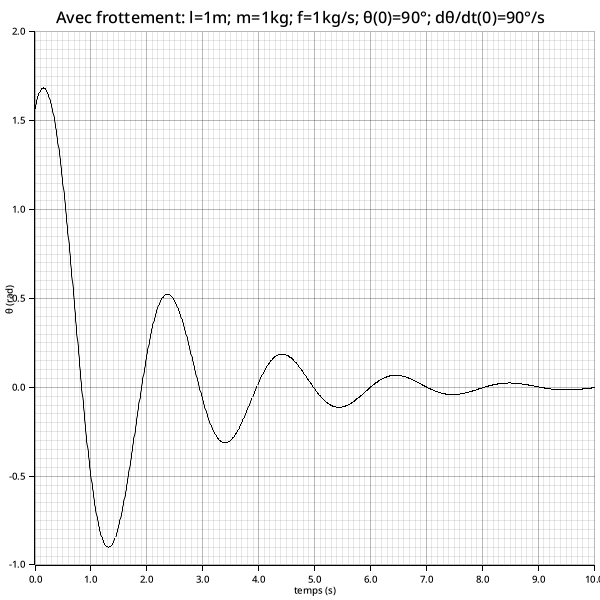
\includegraphics[width=20em]{images/pendule_friction_90_f_vi.png}
        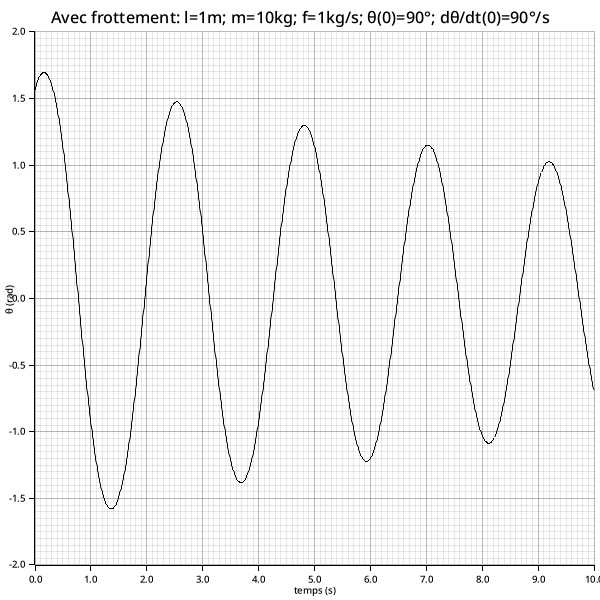
\includegraphics[width=20em]{images/pendule_friction_90_vi_f_m.png}
        \caption{Quelques courbes avec frottements}
      \end{figure}

    
    }

    \question{6}{
      BONUS:
      Il est intéressant de remarquer que la formule de borda n'a pas l'air d'être vérifié si des frottements s'appliquent sur le système:
    
    \begin{figure}[H]
      \centering
      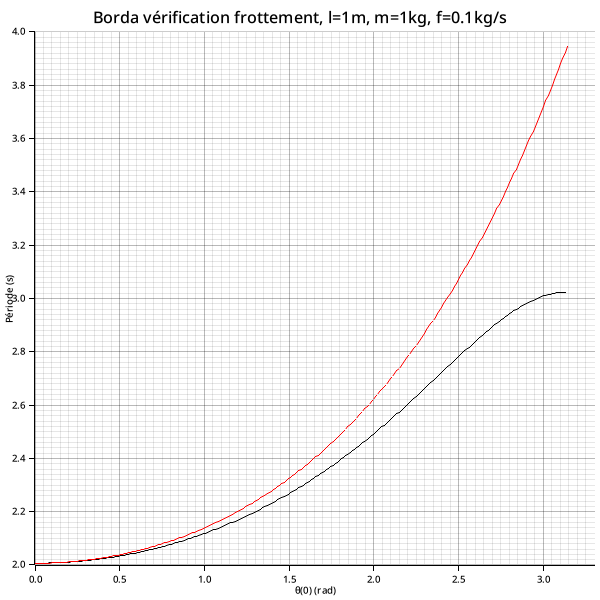
\includegraphics[width=35em]{images/borda_frottement.png}
      \caption{En noir l'approximation numérique. En orange la formule de borda à l'ordre 4}
    \end{figure}
    }
   
  
}


\end{document}
